\documentclass{article}
\usepackage[margin=1.5cm,bottom=2cm]{geometry}
\usepackage{fancyhdr}
\usepackage{graphicx}
\usepackage{amsmath}
\pagestyle{fancy}

\begin{document}
\fancyhead[L]{ 
\includegraphics[width=2cm]{au_logo.png} }
\fancyhead[R]{CPSC 2320: C++ Programming}
\fancyfoot[C]{\thepage}
\vspace*{0cm}
\begin{center}
	{\LARGE \textbf{Midterm Project}}\\
	\vspace{0.25cm}
	{\Large Due: Thursday, October 15}
\end{center}

\section*{Overview}
You are going to write the physics engine for the game \textbf{\textit{Tanks!}}. In this game, a player and an enemy tank are randomly placed on a two-dimensional map. They then take turns firing at one another. The player can toggle the launch velocity and angle before each shot.

\begin{figure}[ht!]
	\centering
	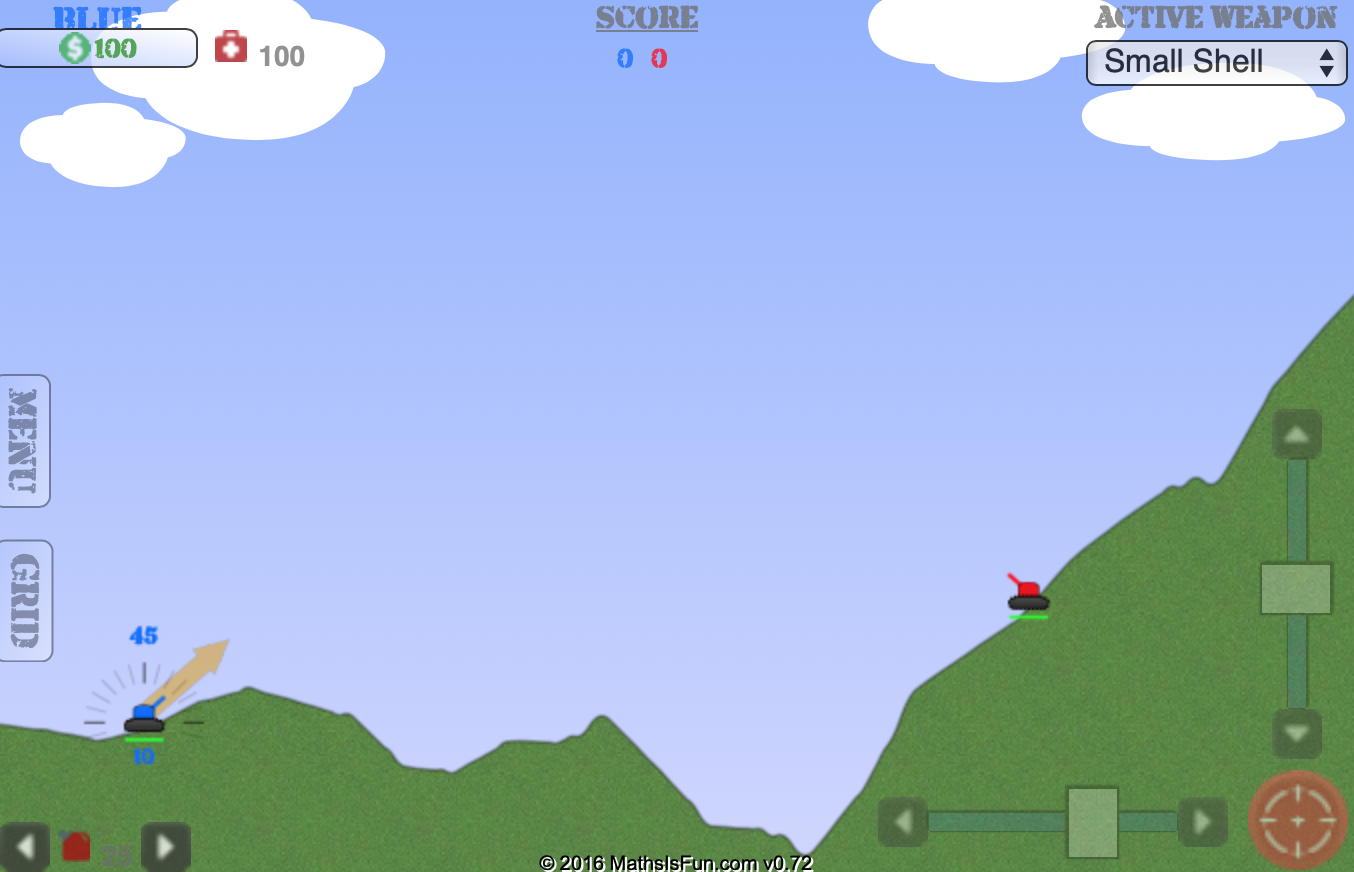
\includegraphics[width=8 cm]{tanks.png}
\end{figure}

\section*{Description}
You will write a program which does the following:
\begin{itemize}
	\item Randomly assign a position ($x$ and $y$ coordinates) for both the player tank and the enemy tank and print these to the console. The enemy tank is \textit{always} to the right of the player.
	\item Tell the user how many of their shells remain (they have 10 to start with)
	\item Prompt the user to enter a launch angle (in degrees) and a launch velocity (in meters per second). Ensure that $-90\leq\theta\leq90^\circ$ and $0<v_0<100$
	\item Calculate the trajectory of the fired shell and determine if the enemy tank was hit.
	\item If the enemy tank was hit, the game is over and the user wins.
	\item Simulate the enemy tank's shot by using a random number to write a function which returns \texttt{true} 10\% of the time. 
	\item The game is over when either the player or enemy tank is destroyed, or if the player runs out of ammunition (the player starts with 10 shells, and loses one each shot). Once the game ends, ask the user if they would like to play again, if they say yes then repeat the process.
\end{itemize}
You must write \textit{at least} the following functions:
\begin{enumerate}
	\item \texttt{double rand\_between(double min, double max)}
	\begin{enumerate}
		\item 	This function returns a random number between min and max (inclusive).
	\end{enumerate}

	\item \texttt{bool check\_hit\_player(double player\_x, double player\_y, double enemy\_x, double enemy\_y, double v0, double theta)}
	\begin{enumerate}
		\item This function will return true if the shell ``hits'' the enemy tank
		\item In order to do this, calculate the $y$ coordinate of the shell at the $x$ location of the enemy tank.
		\begin{enumerate}
			\item First calculate the travel time from the player's tank to the enemy tank: $t=\frac{x_\mathrm{enemy}-x_\mathrm{player}}{v_0\cos{\theta}}$ 
			\item The $y$ position then is: $y_\mathrm{shell}=y_\mathrm{player}+v_0\sin{\theta}t-\frac{1}{2}gt^2$, where $g=9.8$ m/s$^2$ is a global constant
		\end{enumerate}
		\item If $|y_\mathrm{shell}-y_\mathrm{enemy}| \leq 5$ meters, the player's shell has made contact and the function returns \texttt{true}.
	\end{enumerate}
	\item \texttt{bool check\_hit\_enemy()}
	\begin{enumerate}
		\item This function does not actually calculate the trajectory of the enemy tank's shot. 
		\item Assume the enemy has a 10\% chance of hitting the player, and simulate this via a ``dice roll'' with random numbers
	\end{enumerate}
\end{enumerate}
The game loop will consist of the following:
\begin{enumerate}
	\item Randomly generate the x and y positions for both the player and the enemy tanks. Enemy should be to the right of the player.
	\item Tell the user where the tanks are located
	\item Give the user 10 shells to try to hit the enemy.  For each attempt:
	\begin{enumerate}
		\item tell the user how many shells remain
		\item prompt the user to enter the angle (enforce the rule that it is between -90$^\circ$ and +90$^\circ$)
		\item prompt the user to enter the initial velocity (check that it is between 0 and 100)
		\item "fire" the shell and check to see if the enemy tank was hit
		\begin{enumerate}
			\item if so, print "You win!" and stop firing shells
			\item if not, tell the user it was a miss (and how much they missed by)
		\end{enumerate}
	\item let the enemy fire a shell
	\begin{enumerate}
		\item if the player's tank was hit, print "You lose!" and stop firing shells
		\item if not, tell the user it was a miss
	\end{enumerate}
	\end{enumerate}
	\item If the shells have run out, the player loses. 
	\item Ask the user if they want to play again (whether they win or lose).  If so, restart at step 1
\end{enumerate}

\section*{Programming Style Requirements}
\begin{itemize}
	\item files begin with a header comment that includes:
	\begin{itemize}
		\item filename, date, author name, purpose of program
	\end{itemize}
	\item in-code comments:
	\begin{itemize}
		\item each logical section should have a brief description
		\item anything that seems tricky or complicated should be explained
	\end{itemize}
	\item variable declaration:
	\begin{itemize}
		\item declared at the beginning of the function with a name that reflects the purpose
	\end{itemize}
	\item functions:
	\begin{itemize}
		\item declared before main(), defined after main(), include a comment describing purpose
	\end{itemize}
	\item Program exits cleanly
	\begin{itemize}
		\item last line should be return 0;
	\end{itemize}
\end{itemize}
\section*{Sample Output}
\textbf{Sample 1}\\
\texttt{
Welcome to Text Tanks!\\
Your position (x,y):  (19.00, 14.90).\\
Enemy position (x,y): (79.40, 40.10).\\
You have 10 shells remaining.\\
Enter an angle between -90.00 and 90.00 degrees: 45\\
Enter a velocity between 0.00 and 100.00 tank units: 30\\
That was a hit!!  You win!\\
You won!  CONGRATULATIONS!!!\\
Press 'y' to play again, any other key to exit: q\\
}\\
\textbf{Sample 2}\\
\texttt{
Welcome to Text Tanks!\\
Your position (x,y):  (16.40, 26.10).\\
Enemy position (x,y): (81.60, 19.10).\\
You have 10 shells remaining.\\
Enter an angle between -90.00 and 90.00 degrees: 45\\
Enter a velocity between 0.00 and 100.00 tank units: 30\\
Your y-position was off by 25.91\\
That was a miss.\\
The enemy missed you.\\
You have 9 shells remaining.\\
Enter an angle between -90.00 and 90.00 degrees: 45\\
Enter a velocity between 0.00 and 100.00 tank units: 20\\
Your y-position was off by -31.95\\
That was a miss.\\
The enemy missed you.\\
You have 8 shells remaining.\\
Enter an angle between -90.00 and 90.00 degrees: 45\\
Enter a velocity between 0.00 and 100.00 tank units: 25\\
Your y-position was off by 5.54\\
That was a miss.\\
The enemy missed you.\\
You have 7 shells remaining.\\
Enter an angle between -90.00 and 90.00 degrees: 45\\
Enter a velocity between 0.00 and 100.00 tank units: 24\\
That was a hit!!  You win!\\
You won!  CONGRATULATIONS!!!\\
Press 'y' to play again, any other key to exit: q\\
}
\textbf{Sample 3}\\
\texttt{
Welcome to Text Tanks!\\
Your position (x,y):  (23.60, 12.80).\\
Enemy position (x,y): (75.60, 54.80).\\
You have 10 shells remaining.\\
Enter an angle between -90.00 and 90.00 degrees: 45\\
Enter a velocity between 0.00 and 100.00 tank units: 45\\
That was a hit!!  You win!\\
You won!  CONGRATULATIONS!!!\\
Press 'y' to play again, any other key to exit: y\\
Welcome to Text Tanks!\\
Your position (x,y):  (10.60, 30.30).\\
Enemy position (x,y): (89.60, 12.80).\\
You have 10 shells remaining.\\
Enter an angle between -90.00 and 90.00 degrees: 45\\
Enter a velocity between 0.00 and 100.00 tank units: 45\\
Your y-position was off by 66.30\\
That was a miss.\\
The enemy missed you.\\
You have 9 shells remaining.\\
Enter an angle between -90.00 and 90.00 degrees: 45\\
Enter a velocity between 0.00 and 100.00 tank units: 20\\
Your y-position was off by -56.40\\
That was a miss.\\
The enemy missed you.\\
You have 8 shells remaining.\\
Enter an angle between -90.00 and 90.00 degrees: 45\\
Enter a velocity between 0.00 and 100.00 tank units: 30\\
Your y-position was off by 28.54\\
That was a miss.\\
The enemy missed you.\\
You have 7 shells remaining.\\
Enter an angle between -90.00 and 90.00 degrees: 45\\
Enter a velocity between 0.00 and 100.00 tank units: 35\\
Your y-position was off by 46.57\\
That was a miss.\\
The enemy hit you!  You lose!!!!!!!!!!!!!!\\
You lose.  Sorry!\\
Press 'y' to play again, any other key to exit: y\\
Welcome to Text Tanks!\\
Your position (x,y):  (24.40, 72.30).\\
Enemy position (x,y): (74.40, 47.80).\\
You have 10 shells remaining.\\
Enter an angle between -90.00 and 90.00 degrees: \\
(continued)\\
}
\end{document}